\documentclass[a4paper]{article}
\setlength{\parindent}{0pt}

%%%%%%%% CREATE DOCUMENT STRUCTURE %%%%%%%%
%% Language and font encodings
\usepackage[english]{babel}
\usepackage[utf8x]{inputenc}
\usepackage[T1]{fontenc}
%\usepackage{subfig}

%% Sets page size and margins
\usepackage[a4paper,top=3cm,bottom=2cm,left=2cm,right=2cm,marginparwidth=1.75cm]{geometry}

%% Useful packages
\usepackage{amsmath}
\usepackage{graphicx}
\usepackage[colorinlistoftodos]{todonotes}
\usepackage[colorlinks=true, allcolors=blue]{hyperref}
\usepackage{caption}
\usepackage{subcaption}
\usepackage{sectsty}
\usepackage{apacite}
\usepackage{float}
\usepackage{algorithm2e}
\usepackage{titling} 
\usepackage{blindtext}
\usepackage[square,sort,comma,numbers]{natbib}
\usepackage[colorinlistoftodos]{todonotes}
\usepackage{xcolor}
\definecolor{darkgreen}{rgb}{0.0, 0.4, 0.0}

% ToDo: List
\usepackage{enumitem,amssymb}
\newlist{todolist}{itemize}{2}
\setlist[todolist]{label=$\square$}

\usepackage{tikz}
\usepackage{verbatim}
\usetikzlibrary{arrows,shapes}

\definecolor{pblue}{rgb}{0.13,0.13,1}
\definecolor{pgreen}{rgb}{0,0.5,0}
\definecolor{pred}{rgb}{0.9,0,0}
\definecolor{pgrey}{rgb}{0.46,0.45,0.48}

\usepackage{tikz}
\usetikzlibrary{calc,shapes.multipart,chains,arrows}

\usepackage{listings}
\lstset{language=Java,
    showspaces=false,
    showtabs=false,
    breaklines=true,
    showstringspaces=false,
    breakatwhitespace=true,
    commentstyle=\color{pgreen},
    keywordstyle=\color{pblue},
    stringstyle=\color{pred},
    basicstyle=\ttfamily,
    colframe=white!75!black,
    moredelim=[is][\textcolor{pgrey}]{\%\%}{\%\%}
}


%%%%%%%% DOCUMENT %%%%%%%%
\begin{document}

\pgfdeclarelayer{background}
\pgfsetlayers{background,main}

\tikzstyle{starting vertex}=[circle,fill=orange!30,minimum size=20pt,inner sep=0pt]
\tikzstyle{vertex}=[circle,fill=black!30,minimum size=20pt,inner sep=0pt]
\tikzstyle{weight} = [font=\small, black!100]
\tikzstyle{edge} = [draw,line width=0.9pt,-,black!100]

%%%% Title Page
\begin{titlepage}

\newcommand{\HRule}{\rule{\linewidth}{0.5mm}} 							% horizontal line and its thickness
\center 
 
% University
\textsc{\LARGE University of Illinois @ Urbana-Champaign}\\[1cm]

% Document info
\textsc{\Large CI 487: Data Structures for CS Teachers}\\[0.2cm]
\textsc{\large }\\[1cm] 										% Course Code
\HRule \\[0.8cm]
{ \huge \bfseries Implementation \#6:\\\vspace{0.1cm}Implementing a Generic Graph}\\[0.7cm]								% Assignment
\HRule \\[0.8cm]

\vfill
\begin{minipage}{0.49\textwidth}
    \begin{figure}[H]
\centering
\begin{tikzpicture}[scale=1.5, auto,swap]

    \foreach \pos/\name in {{(0,1)/a}, {(2,1)/b}, {(4,1)/c},
                            {(0,0)/d}, {(3,0)/e}, {(2,-1)/f}, {(4,-1)/g}}
        \node[vertex] (\name) at \pos {};

    \foreach \source/ \dest /\weight in {b/a/7, c/b/8,d/a/5,d/b/9,
                                         e/b/7, e/c/5,e/d/15,
                                         f/d/6,f/e/8,
                                         g/e/9,g/f/11}
        \draw[->, edge] (\source) -- node[weight] {$\weight$} (\dest);

\end{tikzpicture}
\end{figure}





\end{minipage}
\hfill
\begin{minipage}{0.49\textwidth}
    \begin{figure}[H]
\centering
\begin{tikzpicture}[scale=1.5, auto,swap]

    \foreach \pos/\name in {{(0,1)/a}, {(2,1)/b}, {(4,1)/c},
                            {(0,0)/d}, {(3,0)/e}, {(2,-1)/f}, {(4,-1)/g}}
        \node[vertex] (\name) at \pos {};

    \foreach \source/ \dest in {b/a, c/b,d/a,d/b,
                                         e/b,e/c,e/d,
                                         f/d,f/e,
                                         g/e,g/f}
        \draw[->, edge] (\source) -- (\dest);

\end{tikzpicture}
\end{figure}

\end{minipage}
\vfill
\begin{minipage}{0.49\textwidth}
    \begin{figure}[H]
\centering
\begin{tikzpicture}[scale=1.5]

    \foreach \pos/\name in {{(0,1)/a}, {(2,1)/b}, {(4,1)/c},
                            {(0,0)/d}, {(3,0)/e}, {(2,-1)/f}, {(4,-1)/g}}
        \node[vertex] (\name) at \pos {};

    \foreach \source/ \dest in {b/a/7, c/b/8,d/a/5,d/b/9,
                                         e/b/7, e/c/5,e/d/15,
                                         f/d/6,f/e/8,
                                         g/e/9,g/f/11}
        \draw[-{>},line width=0.9pt] (\source) to (\dest);
\end{tikzpicture}
\end{figure}





\end{minipage}
\hfill
\begin{minipage}{0.49\textwidth}
    \resizebox{0.75\textwidth}{!}{
\begin{tikzpicture}[scale=1.5, auto,swap]

    \foreach \pos/\name in {{(0,1)/a}, {(2,1)/b}, {(4,1)/c},
                            {(0,0)/d}, {(3,0)/e}, {(2,-1)/f}, {(4,-1)/g}}
        \node[vertex] (\name) at \pos {\name};

    \foreach \source/ \dest /\weight in {b/a/7, c/b/8,d/a/5,d/b/9,
                                         e/b/7, e/c/5,e/d/15,
                                         f/d/6,f/e/8,
                                         g/e/9,g/f/11}
        \draw[-{>},line width=0.9pt] (\source) -- node[weight] {$\weight$} (\dest);

\end{tikzpicture}}

\end{minipage}
\vfill

\vfill 
\end{titlepage}

%%\begin{abstract}
%%Your abstract.
%%\end{abstract}

%%%% SECTIONS
%% Section 1
\section{Objectives and Overview}

The objective of this lab will be the following:
\begin{enumerate}
    \item Construct a generic graph with an adjacency list.
    \item The graph constructor and implementation should allow for weighted/unweighted and directed/undirect construction and operations.
    \item The graph should support Breadth-First Search (BFS) and Depth-First Search(DFS) from a given starting vertex.
\end{enumerate}
To construct an generic graph that supports operations for a generic graph represented using an \textit{adjacency list}. 

\section{Checkpoint 1}

\subsection{Adjacencly List  Design Details}

Lets begin this lab with a general description of the algorithms and general
design of the graph we will be building.

\subsubsection{Adjacency List}
\begin{figure}[H]
    \centering
    \begin{tikzpicture}[list/.style={rectangle split, rectangle split parts=2, draw, rectangle split verical}, start chain]

            \node[list,on chain] (A) {value=12 \nodepart{second} weight=1};

    \end{tikzpicture}\\
    \caption{A visual representation of an edge}
    \label{fig:edge}
\end{figure}

Our implementation of an adjacency list will be composed of a HashMap with
vertices as keys and edge lists as values. As you will see in
Section~\ref{sec:edge}, an edge is composed of two attributes, a weight and the
vertex containing a destination (Figure~\ref{fig:edge}). The following is an
example of how a graph is represented by an adjacency matrix.\\

\begin{minipage}{0.4\textwidth}
    {\renewcommand{\arraystretch}{1.2}% for the vertical padding}
    \begin{tabular}{| c | l |}
        \hline
        Key & Value \\
        \hline
        a & \rule[11.2ex]{0pt}{0pt}  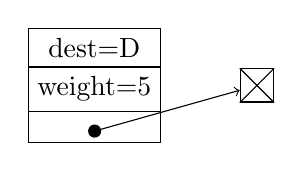
\begin{tikzpicture}[list/.style={rectangle split, rectangle split parts=3, draw}, start chain]

                \foreach \x/ \w in {D/5}{
                    \node[list,on chain] (\x) {dest=\x \nodepart{second} weight=\w};
                }


                \node[on chain,draw,inner sep=6pt] (N) {};
                \draw (N.north east) -- (N.south west);
                \draw (N.north west) -- (N.south east);


                \foreach \s/ \d in {D/N}{
                    \draw[*->] let \p1 = (\s.three), \p2 = (\s.three) in (\x1,\y2) -- (\d);
                }

        \end{tikzpicture}
        \\ \hline
        b & \rule[11.2ex]{0pt}{0pt} 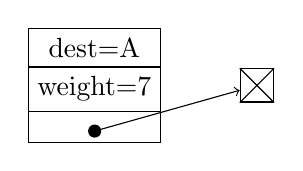
\begin{tikzpicture}[list/.style={rectangle split, rectangle split parts=3, draw}, start chain]

                \foreach \x/ \w in {A/7}{
                    \node[list,on chain] (\x) {dest=\x \nodepart{second} weight=\w};
                }


                \node[on chain,draw,inner sep=6pt] (N) {};
                \draw (N.north east) -- (N.south west);
                \draw (N.north west) -- (N.south east);


                \foreach \s/ \d in {A/N}{
                    \draw[*->] let \p1 = (\s.three), \p2 = (\s.three) in (\x1,\y2) -- (\d);
                }

        \end{tikzpicture}
        \\ \hline
        c & \rule[11.2ex]{0pt}{0pt} 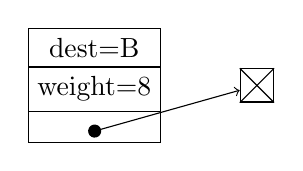
\begin{tikzpicture}[list/.style={rectangle split, rectangle split parts=3, draw}, start chain]

                \foreach \x/ \w in {B/8}{
                    \node[list,on chain] (\x) {dest=\x \nodepart{second} weight=\w};
                }


                \node[on chain,draw,inner sep=6pt] (N) {};
                \draw (N.north east) -- (N.south west);
                \draw (N.north west) -- (N.south east);


                \foreach \s/ \d in {B/N}{
                    \draw[*->] let \p1 = (\s.three), \p2 = (\s.three) in (\x1,\y2) -- (\d);
                }
        \end{tikzpicture}
        \\ \hline
        d & \rule[11.2ex]{0pt}{0pt} 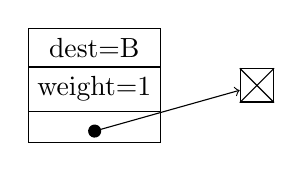
\begin{tikzpicture}[list/.style={rectangle split, rectangle split parts=3, draw}, start chain]

                \foreach \x/ \w in {B/1}{
                    \node[list,on chain] (\x) {dest=\x \nodepart{second} weight=\w};
                }


                \node[on chain,draw,inner sep=6pt] (N) {};
                \draw (N.north east) -- (N.south west);
                \draw (N.north west) -- (N.south east);


                \foreach \s/ \d in {B/N}{
                    \draw[*->] let \p1 = (\s.three), \p2 = (\s.three) in (\x1,\y2) -- (\d);
                }

        \end{tikzpicture}
        \\ \hline
        e & \rule[11.2ex]{0pt}{0pt} 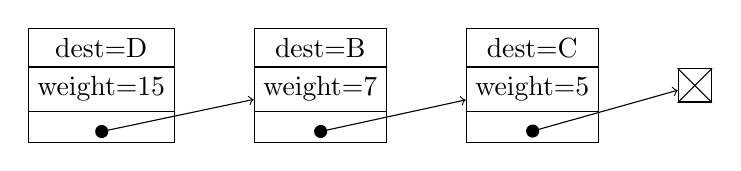
\begin{tikzpicture}[list/.style={rectangle split, rectangle split parts=3, draw}, start chain]

                \foreach \x/ \w in {D/15, B/7, C/5}{
                    \node[list,on chain] (\x) {dest=\x \nodepart{second} weight=\w};
                }


                \node[on chain,draw,inner sep=6pt] (N) {};
                \draw (N.north east) -- (N.south west);
                \draw (N.north west) -- (N.south east);


                \foreach \s/ \d in {D/B, B/C, C/N}{
                    \draw[*->] let \p1 = (\s.three), \p2 = (\s.three) in (\x1,\y2) -- (\d);
                }



        \end{tikzpicture}
        \\ \hline

    \end{tabular}
    }
\end{minipage}
\hfill
\begin{minipage}{0.4\textwidth}
\begin{figure}[H]
\centering
\begin{tikzpicture}[scale=0.7, auto,swap]

    \node[starting vertex] (a) at (-5,2) {a};
    \foreach \pos/\name in {{(-2,5)/b}, {(2,2)/c},
                            {(-3,-2)/d}, {(0,0)/e}}
        \node[vertex] (\name) at \pos {$\name$};

    \foreach \source/ \dest/ \weight in {b/a/7, c/b/8,a/d/5,
                                         e/b/7, e/c/5,e/d/15,
                                         d/b/1
                                         }
        \draw[-{>},line width=0.9pt] (\source) -- node[weight] {$\weight$} (\dest);
\end{tikzpicture}
\end{figure}
\end{minipage}

\\
\vspace{0.25cm}



\subsection{Edge}\label{sec:edge}
Just as with the simpler graphs we covered this semester (e.g., Trees,
LinkedLists) our graph must have some set of basic units.  For graphs these
units are the vertecies and the edges. Since we are implementing our graph with
an adjacency list we will need a method of indicating to which vertices a
vertex is connected and what the weight of that edge is, if applicable.  As
such, we will be building an inner class \lstinline|Edge<E>| that stores this
information on the destination and the weight. The adjacency list that results 
from this will be a lists of edges that exist with respect to a given vertex. 
As you will see in the starter files, this class is inner class within the 
encompassing \lstinline|ListGraph<E>| class since it has little utility
outside the context of constructing a list graph. In this case \lstinline|E|
will be the type of our vertecies since we are represnting the graph with
just an edgelist.

\subsubsection{Attributes}

The following attributes will be used for representing the edges of our class:
\begin{enumerate}
    \item \lstinline|final int weight|
    \item \lstinline|final E dest|  
\end{enumerate}
Both of these attributes should be declared as \lstinline|final| since, once
set, we will not be changing the values associated with an instance of an
\lstinline|Edge|.

\subsubsection{Constructors}

\paragraph{\lstinline|public Edge(E dest) { ... }|}: This constructor will be
used for the creation of edges for unweighted graphs; hence, the reason for the
absence of an integer parameter indicating the weight of the edge. It should
therefore set the \lstinline|weight| attribute to zero when a new edge is
instantiated using this constructor. The \lstinline|dest| parameter is generic
and will contain a reference to the destination object.

\paragraph{\lstinline|public Edge(E dest, int weight) { ... }|} This
constructor is similar to the former one but adds a primitive integer parameter
\lstinline|weight|. As such, this constructor will be used for the construction
of weighted edges and should set the \lstinline|dest| and \lstinline|weight| 
attributes of the object equal to the parameters passed through the function.


\subsection{ListGraph}
\subsubsection{Attributes}

\begin{enumerate}
    \item \lstinline|private final boolean directed| 
    \item \lstinline|private final boolean weighted|
    \item \lstinline|private Map<E, List<Edge<E>>> map|
\end{enumerate}

The purpose of the \lstinline|directed| and \lstinline|weighted| is to direct
the control flow of methods relating to the addition and removal of edges. 
The map is the data-structure we will be using to represent our adacency list.
Each vertex \lstinline|E| will be associated with a \lstinline|List| of 
\lstinline|Edge| instances. 

\subsubsection{Constructor}

\paragraph{\lstinline|public ListGraph(boolean directed, boolean weighted) \{
... \}|}: This is the only constructor we will have for this class since
control flow of variations on the graph will be handled via the two parameters.
It should set the \lstinline|directed| and \lstinline|weighted| attributes
equal to the values passed in as parameter s to the constructor. It should also
create a new, empty instance of \lstinline|Map| that associates vertecies of
\lstinline|E| with and edge list of \lstinline|List<Edge<E>>|.



\subsubsection{Vertex Methods}

\paragraph{\lstinline|public void addVertex(E vertex) { ... }|}: The add
vertex method should create a new entry in the \lstinline|map| and associate it
with a new instance of an empty \lstinline|List| of \lstinline|Edges|.

\paragraph{\lstinline|public void removeVertex(E vertex) { ... }|}: The 
remove vertex function should do two things: (1) remove the given vertex
and it's associated list of edges and (2) search through all other 
edge lists in \lstinline|map| and all those edges with the given 
vertex as the \lstinline|dest|.

%\noindent \textit{Hint:} Look into the
%\href{https://docs.oracle.com/javase/8/docs/api/java/util/Collection.html#removeIf-java.util.function.Predicate-}{\lstinline|removeIf|} 
%function for the \lstinline|List| interface in the Java documentation. It can
%be used to reduce the complexity of the second objective of the
%\lstinline|removeVertex| function.

\paragraph{\lstinline|public Set<E> getVertecies() { ... }|}: This 
should return a list of the vertecies currently in \lstinline|map|. \\

\noindent\textit{Hint:} This method should be one line of code that returns
the keyset from the map. Refer to the \lstinline|HashMap| documentation for
which method can accomplish this.

\subsubsection{Edge Methods}

The following two methods will handle the addition of edges to the graph. 
\begin{enumerate}
    \item \lstinline|public void addEdgeUnweighted(E source, E dest) { ... }|
    \item \lstinline|public void addEdgeWeighted(E source, E dest, int weight) { ... }|
\end{enumerate}
Each of these methods should first check if both the given \lstinline|source|
and the \lstinline|dest| should be in the \lstinline|map|. If they are, it
should instantiate a new edge, \textit{taking care to call the appropriate
constructor}, and add the edge to \lstinline|source|'s associate edge list in
\lstinline|map|. If the graph is undirected, it should follow a similar process
to create an edge from \lstinline|dest| to \lstinline|source|.


\paragraph{\lstinline|public void removeEdge(E source, E dest) \{ ... \}|}: 
This method should remove the edge from \lstinline|source| to \lstinline|dest|
and, if the graph graph is undirected, from \lstinline|dest| to \lstinline|source|.

\paragraph{\lstinline|public List<Edge<E>> getEdges(E vertex) \{ ... \}|}: This
is a getter method that retrieves the edgelist associated with a given vertex.\\

\noindent\textit{Hint:} This method should be one line of code that returns the
list associated with a vertex. Refer to the \lstinline|HashMap| documentation
for which method can accomplish this.




\section{Checkpoint 2}

For the second checkpoint you will be implementing both a breadth first and
depth first search. In donig so, you will complete the following two methods:

\paragraph{\lstinline|public List<E> bfs(T source) \{ ... \}|}: This function
should perform the BFS function described in Section~\ref{sec:bfs} begining at the
\lstinline|source| node passed in as a parameter, collect a list of references
to each of the objects along the way, and return that list once the algorithm
has completed.

\paragraph{\lstinline|public List<E> dfs(T vertex) \{ ... \}|}: This method 
should perform the DFS function described in Section~\ref{sec:dfs} begining at the
\lstinline|source| node passed in as a parameter, collect a list of references
to each of the objects along the way, and return that list once the algorithm
has completed.




\subsubsection{Breadth-First Search}\label{sec:bfs}
\begin{minipage}{0.49\textwidth}
\RestyleAlgo{ruled} 
\begin{algorithm}[H]
    \caption{Breadth First Search}\label{alg:bfs}
    \DontPrintSemicolon
    \SetKwFunction{FBFS}{BFS}
    \SetKwProg{Fn}{Function}{}{}
    \Fn{\FBFS{G, Source}}{
        \For{ u $\in$ G.Vertex}{
            u.visited $\gets$ null\;
        }
        Q $\gets \emptyset$\; 
        Q.enqueue(Source)\;
        \While{Q $\neq \emptyset$}{
            u $\gets$ Q.dequeue()\;
            \If{u is visited}{
                continue\;
            }
            u.visited $\gets$ true\;
            \For{edge $\in$ G.Adj[u]}{
                \If{edge.dest is not visited}{
                    Q.enqueue(edge.dest)\;
                }
            }
        }
    }
\end{algorithm}
\textit{Note: the traversals shown on the right will vary depending on the order in which vertecies are pushed to the queue.}
\end{minipage}
\hfill
% NOTE: Credit for this goes to -> https://texample.net/tikz/examples/prims-algorithm/
\begin{minipage}{0.46\textwidth}
\textbf{Results for Directed Graph:}
\begin{figure}[H]
\centering
\begin{tikzpicture}[scale=1.5]

    \node[starting vertex] (a) at (0, 1) {a};
    \foreach \pos/\name in {{(2,1)/b}, {(4,1)/c},
                            {(0,0)/d}, {(3,0)/e}, {(2,-1)/f}, {(4,-1)/g}}
        \node[vertex] (\name) at \pos {$\name$};

    \foreach \source/ \dest in {a/b/7, c/b/8,a/d/5,d/b/9,
                                         e/b/7, e/c/5,e/d/15,
                                         f/d/6,f/e/8,
                                         g/e/9,g/f/11}
        \draw[-{>[scale=4.5]},line width=0.9pt] (\source) to (\dest);
\end{tikzpicture}
\end{figure}
\footnotesize{\textbf{Traversal:}} a b d\\
\hline
\vspace{0.2cm}
\textbf{Results for Undirected Graph:}
\begin{figure}[H]
\centering
\begin{tikzpicture}[scale=1.5, auto,swap]

    \node[starting vertex] (a) at (0, 1) {a};
    \foreach \pos/\name in {{(2,1)/b}, {(4,1)/c},
                            {(0,0)/d}, {(3,0)/e}, {(2,-1)/f}, {(4,-1)/g}}
        \node[vertex] (\name) at \pos {$\name$};

    \foreach \source/ \dest in {b/a, c/b,d/a,d/b,
                                         e/b,e/c,e/d,
                                         f/d,f/e,
                                         g/e,g/f}
        \draw[->, edge] (\source) -- (\dest);

\end{tikzpicture}
\end{figure}
\footnotesize{\textbf{Traversal:}} a b d e c f g
\end{minipage}

\vspace{0.25cm}\\

\noindent Algorithm~\ref{alg:bfs} presents the iterative approach you will take
for implementing BFS from a given source node. The purpose of the variables 
used in that psudeocode are as follows:
\begin{itemize}
    \item \lstinline|G| is the graph on which the alorithm will operate.
    \item \lstinline|Source| is our starting vertex
    \item \lstinline|Q| is a \textit{queue} that contains the ondes under consideration for traversal. We initiallize it to empty, add the starting vertex, and then begin the traversal.
\end{itemize}

As with the other psudeocode we've used in this class, it is important to note
that the psudeocode is simply a general set of instructions on how the solution
should be structured. Your implementation should follow it in spirit but
\textit{will not be a direct translation of the psudeocode to Java}. Noteably,
your vertecies will not have a \lstinline|visited| attribute. You will instead
need to use some other inbuilt data structure (e.g., \lstinline|Map|) to keep
track of whether or not a node has been visited.



\subsubsection{Depth-First Search}\label{sec:dfs}
\begin{minipage}{0.49\textwidth}
\RestyleAlgo{ruled} 
\begin{algorithm}[H]
    \caption{Depth First Search}\label{alg:dfs}
    \DontPrintSemicolon
    \SetKwFunction{FDFS}{DFS}
    \SetKwProg{Fn}{Function}{}{\KwRet}
    \Fn{\FDFS{G, Source}}{
        \For{ u $\in$ G.Vertex}{
            u.visited $\gets$ false\;
        }
        S $\gets \emptyset$\; 
        S.push(Source)\;
        \While{S $\neq \emptyset$}{
            u $\gets$ S.pop()\;
            \If{u is visited}{
                continue\;
            }
            u.visited $\gets$ true\;
            \For{edge $\in$ G.Adj[u]}{
                \If{edge.dest is not visited}{
                    S.add(edge.dest)\;
                }
            }
        }
    }
\end{algorithm}
\textit{Note: the traversals shown on the right will vary depending on the order in which vertecies are pushed to the stack.}
\end{minipage}
\hfill
% NOTE: Credit for this goes to -> https://texample.net/tikz/examples/prims-algorithm/
\begin{minipage}{0.46\textwidth}
\textbf{Results for Directed Graph:}
\begin{figure}[H]
\centering
\begin{tikzpicture}[scale=1.5]

    \node[starting vertex] (a) at (0, 1) {a};
    \foreach \pos/\name in {{(2,1)/b}, {(4,1)/c},
                            {(0,0)/d}, {(3,0)/e}, {(2,-1)/f}, {(4,-1)/g}}
        \node[vertex] (\name) at \pos {$\name$};

    \foreach \source/ \dest in {a/b/7, c/b/8,a/d/5,d/b/9,
                                         e/b/7, e/c/5,e/d/15,
                                         f/d/6,f/e/8,
                                         g/e/9,g/f/11}
        \draw[-{>[scale=4.5]},line width=0.9pt] (\source) to (\dest);
\end{tikzpicture}
\end{figure}
\footnotesize{\textbf{Traversal:}} a b d\\
\hline
\vspace{0.2cm}
\textbf{Results for Undirected Graph:}
\begin{figure}[H]
\centering
\begin{tikzpicture}[scale=1.5, auto,swap]

    \node[starting vertex] (a) at (0, 1) {a};
    \foreach \pos/\name in {{(2,1)/b}, {(4,1)/c},
                            {(0,0)/d}, {(3,0)/e}, {(2,-1)/f}, {(4,-1)/g}}
        \node[vertex] (\name) at \pos {$\name$};

    \foreach \source/ \dest in {a/b/7, c/b/8,d/a/5,d/b/9,
                                         e/b,e/c,e/d,
                                         f/d,f/e,
                                         g/e,g/f}
        \draw[->, edge] (\source) -- (\dest);

\end{tikzpicture}
\end{figure}
\footnotesize{\textbf{Traversal:}} a d f g e b c
\end{minipage}\\

\vspace{0.25cm}\\

\noindent Algorithm~\ref{alg:dfs} presents the iterative approach you will take
for implementing DFS from a given source node. This is very similar to BFS however there are a few new variables in the psudeocode
\begin{itemize}
    \item \lstinline|G| is the graph on which the alorithm will operate.
    \item \lstinline|Source| is our starting vertex
    \item \lstinline|S| is a \textit{stack} that contains the node still under consideration for traversal.
\end{itemize}

Again, your implementation should follow it in spirit but \textit{will not be a
direct translation of the psudeocode to Java}. As with the BFS, your vertecies
will not have a \lstinline|visited| attribute. You will instead need to use
some other inbuilt data structure (e.g., \lstinline|Map|) to keep track of
whether or note a node has been visited.


\newpage
\section{Checklist}
\begin{itemize}
    \item Edge 
        \begin{todolist}
            \item The class has a \lstinline|weight| and \lstinline|attribute| 
            \item The class has two constructors, one for weighted edges and the other for unweighted.
        \end{todolist}
    \item ListGraph 
        \begin{todolist}
            %\item The \lstinline|directed|, \lstinline|weighted|, and \lstinline|map| attributes are present and declared with the proper modifiers.
            %\item The constructor has been implemented according to spec.
            \item The following methods have been implemented:
            \begin{todolist}
                \item \lstinline|addVertex|
                \item \lstinline|removeVertex|
                \item \lstinline|getVertecies|
                \item \lstinline|addEdgeUnweighted|
                \item \lstinline|addEdgeWeighted|
                \item \lstinline|removeEdge|
                \item \lstinline|getEdges|
                \item \lstinline|bfs|
                \item \lstinline|dfs|
            \end{todolist}
        \end{todolist}
\end{itemize}


%\section{Rubric}


%%\newpage
%%\bibliographystyle{apacite}
%%\bibliography{sample}

\end{document}
